% =============================================================================
% 20-bab2.tex — BAB II LANDASAN TEORI
% Patches: C2 (4 roles), C4 (bcryptjs), C5 (5 scoring functions),
%          C6 (2-job CI), C9 (5 auth tiers), C10 (proxy.ts)
% =============================================================================
\chapter{LANDASAN TEORI}
\label{chap:landasan-teori}

Bab ini memaparkan landasan teori yang menjadi dasar ilmiah dan teknis dalam perancangan serta implementasi Platform Asesmen Digital CHP. Sesuai dengan fokus penulis pada arsitektur sistem, pengembangan \textit{backend}, dan pengujian perangkat lunak, teori yang dibahas mencakup rekayasa perangkat lunak dengan metodologi Agile, arsitektur sistem web modern berbasis Next.js, pengembangan \textit{backend} dengan tRPC dan PostgreSQL, sistem autentikasi dan otorisasi, strategi pengujian perangkat lunak, serta keamanan dan privasi data.

% ─────────────────────────────────────────────────────────────────────────────
\section{Rekayasa Perangkat Lunak}
\label{sec:rekayasa-pl}

Rekayasa Perangkat Lunak (\textit{Software Engineering}) adalah disiplin ilmu teknik yang berkaitan dengan semua aspek produksi perangkat lunak, mulai dari tahap spesifikasi awal sistem hingga pemeliharaan sistem setelah digunakan (Sommerville 2016). Rekayasa perangkat lunak mencakup manajemen proyek, proses pengembangan, metode teknis, dan penggunaan alat (\textit{tools}) yang tepat guna menghasilkan perangkat lunak yang dapat diandalkan, efisien, dan memenuhi kebutuhan penggunanya.

Proses rekayasa perangkat lunak pada umumnya melibatkan empat aktivitas fundamental yang saling berkaitan, yaitu: (1) spesifikasi perangkat lunak, yaitu pendefinisian fungsionalitas dan kendala operasi sistem; (2) pengembangan perangkat lunak, yaitu perancangan dan pemrograman sistem sesuai spesifikasi; (3) validasi perangkat lunak, yaitu pemastian bahwa sistem memenuhi kebutuhan pengguna; serta (4) evolusi perangkat lunak, yaitu modifikasi sistem sebagai respons terhadap perubahan kebutuhan. Pada proyek Platform CHP, keempat aktivitas ini dilaksanakan secara iteratif dalam kerangka metodologi Agile.

\subsection{Model Proses: Metodologi Agile}
\label{subsec:agile}

Model proses perangkat lunak mendefinisikan pendekatan yang digunakan untuk mengorganisasi dan mengelola aktivitas pengembangan. Dalam proyek ini, model Agile iteratif dan inkremental dipilih sebagai kerangka kerja pengembangan. Agile adalah sekumpulan nilai dan prinsip yang diformulasikan dalam \textit{Agile Manifesto} (2001), yang menekankan respons terhadap perubahan di atas mengikuti rencana yang kaku, kolaborasi erat dengan pelanggan di atas negosiasi kontrak, dan penyerahan perangkat lunak yang berfungsi di atas dokumentasi yang ekstensif.

Manifestasi Agile yang digunakan dalam proyek ini adalah Scrum, sebuah kerangka kerja manajemen proyek yang mengorganisasi pekerjaan ke dalam siklus waktu tetap yang disebut \textit{sprint} (Schwaber dan Sutherland 2020). Setiap \textit{sprint} pada proyek CHP berdurasi dua minggu. Pada setiap akhir \textit{sprint}, tim menghasilkan \textit{increment} (versi perangkat lunak yang siap didemonstrasikan dan berpotensi untuk dirilis). Dalam konteks KP ini, pertemuan dua mingguan dengan Ibu Astin selaku pemilik proyek berfungsi sebagai sesi \textit{sprint review}, di mana demonstrasi fitur yang telah diimplementasikan disampaikan untuk mendapatkan umpan balik langsung.

Pemilihan Agile untuk proyek ini didasari tiga pertimbangan utama:

\begin{enumerate}[leftmargin=2cm]
  \item Jadwal tetap 12 minggu menuntut penyerahan fitur secara inkremental, sehingga pemangku kepentingan dapat menggunakan dan memberikan umpan balik terhadap fitur yang sudah selesai sembari fitur lain masih dikembangkan.
  \item Kebutuhan instrumen psikometri dari tim psikologi dapat berevolusi selama pengembangan, dan Agile mengakomodasi perubahan ini tanpa memerlukan renegosiasi kontrak formal.
  \item Tim kecil yang terdiri atas dua pengembang cocok dengan prinsip Agile yang mengutamakan komunikasi langsung dan minimalisasi birokrasi proses.
\end{enumerate}

% ─────────────────────────────────────────────────────────────────────────────
\section{Arsitektur Sistem Web Modern}
\label{sec:arsitektur-web}

Arsitektur sistem web mengacu pada struktur tingkat tinggi dari sebuah aplikasi web yang mendefinisikan bagaimana komponen-komponen penyusunnya diorganisasi, berinteraksi, dan berkomunikasi satu sama lain.

\subsection{Arsitektur Tiga Lapisan}
\label{subsec:three-tier}

Arsitektur tiga lapisan (\textit{three-tier architecture}) adalah pola arsitektur yang membagi aplikasi menjadi tiga lapisan logis yang terpisah: lapisan presentasi (\textit{presentation tier}), lapisan aplikasi (\textit{application tier}), dan lapisan data (\textit{data tier}). Pemisahan ini menerapkan prinsip \textit{separation of concerns} yang memungkinkan setiap lapisan untuk dikembangkan, diuji, dan diskalakan secara independen.

Pada Platform Asesmen Digital CHP, ketiga lapisan diimplementasikan sebagai berikut:

\begin{enumerate}[leftmargin=2cm]
  \item Lapisan Presentasi: Komponen React dengan \textit{React Server Components} (RSC), Tailwind CSS, dan shadcn/ui yang menghasilkan antarmuka pengguna interaktif dan responsif.
  \item Lapisan Aplikasi: \textit{Router} tRPC, \textit{scoring engine}, \textit{middleware} autentikasi, dan \textit{Server Actions} yang mengandung seluruh logika bisnis sistem.
  \item Lapisan Data: PostgreSQL yang diakses melalui Drizzle ORM sebagai sumber data utama, dengan Upstash Redis sebagai lapisan \textit{caching} dan \textit{rate limiting}.
\end{enumerate}

Gambar~\ref{fig:arsitektur-3-tier} mengilustrasikan diagram arsitektur tiga lapisan Platform CHP.

\begin{figure}[htbp]
  \centering
  \includegraphics[width=\textwidth]{figures/gambar_2_1_arsitektur_tiga_lapisan.png}
  \caption{Diagram Arsitektur Tiga Lapisan Platform Asesmen Digital CHP}
  \label{fig:arsitektur-3-tier}
\end{figure}

\subsection{Next.js dan \textit{React Server Components}}
\label{subsec:nextjs}

Next.js adalah \textit{meta-framework} berbasis React yang menyediakan fondasi lengkap untuk membangun aplikasi web \textit{full-stack} modern (Vercel 2026). Proyek ini menggunakan Next.js 16 dengan \textit{App Router} yang membawa pergeseran arsitektural signifikan melalui \textit{React Server Components} (RSC).

RSC adalah paradigma \textit{rendering} yang memungkinkan komponen React dieksekusi dan di-\textit{render} secara eksklusif di sisi server, tanpa mengirimkan kode JavaScript komponen tersebut ke \textit{browser} klien. Implikasi praktis RSC untuk Platform CHP adalah pengurangan ukuran \textit{bundle} JavaScript yang dikirim ke \textit{browser} peserta tes. Komponen yang hanya membaca data, seperti halaman katalog tes, halaman informasi, dan halaman hasil, di-\textit{render} di server tanpa mengirimkan kodenya ke klien. Hanya komponen yang memerlukan interaktivitas, seperti formulir asesmen dan tombol navigasi, yang ditandai dengan direktif \texttt{"use client"} dan dikirim ke \textit{browser}.

% ─────────────────────────────────────────────────────────────────────────────
\section{TypeScript dan Keamanan Tipe}
\label{sec:typescript}

TypeScript adalah bahasa pemrograman \textit{open-source} yang dikembangkan oleh Microsoft sebagai \textit{superset} dari JavaScript. TypeScript menambahkan sistem pengetikan statis (\textit{static type system}) di atas JavaScript, sehingga setiap variabel, parameter fungsi, dan nilai kembalian dapat diberikan anotasi tipe eksplisit.

\subsection{Signifikansi TypeScript dalam Proyek CHP}
\label{subsec:typescript-chp}

Sebuah studi berskala besar terhadap 85 proyek web oleh Bogner dan Merkel (2022) menunjukkan bahwa penggunaan TypeScript menurunkan densitas \textit{code smell} sebesar 34\% dan mengurangi kompleksitas kognitif sebesar 28\% dibandingkan JavaScript murni (Bogner dan Merkel 2022). Studi lain (arXiv 2026) mengungkap bahwa pengetikan statis mengubah lanskap kegagalan pada aplikasi modern: mayoritas \textit{bug} dalam proyek ekosistem TypeScript bersumber dari kesalahan konfigurasi \textit{toolchains}, penyalahgunaan integrasi antarmuka API, dan kegagalan penanganan status asinkron.

Pada Platform CHP, TypeScript digunakan di seluruh \textit{codebase} dengan konfigurasi \texttt{strict: true} yang mengaktifkan pemeriksaan tipe paling ketat. Setiap prosedur tRPC mendefinisikan skema masukan dan keluaran menggunakan pustaka validasi Zod, yang secara otomatis menghasilkan tipe TypeScript.

% ─────────────────────────────────────────────────────────────────────────────
\section{Backend dan Basis Data}
\label{sec:backend-db}

\subsection{PostgreSQL dan Basis Data \textit{Serverless}}
\label{subsec:postgresql}

PostgreSQL adalah sistem manajemen basis data relasional \textit{open-source} yang dikenal karena kepatuhannya terhadap standar SQL, ekstensibilitas, dan dukungan terhadap tipe data kompleks seperti JSONB (PostgreSQL Global Development Group 2026). Platform CHP menggunakan PostgreSQL 17 melalui layanan \textit{serverless} Neon yang memisahkan komputasi dari penyimpanan, memungkinkan basis data untuk diskalakan ke nol saat tidak ada permintaan dan aktif kembali dalam hitungan milidetik.

\subsection{Drizzle ORM dan Perancangan Skema}
\label{subsec:drizzle}

Drizzle ORM adalah ORM TypeScript generasi baru yang berfilosofi ``SQL-\textit{first}'', sintaksis API-nya dirancang semirip mungkin dengan SQL namun sepenuhnya aman secara tipe (Drizzle Team 2026). Skema basis data Platform CHP dirancang untuk mendukung instrumen psikometri yang fleksibel. Tabel~\ref{tab:ringkasan-skema} menyajikan ringkasan tabel-tabel utama.

\begin{table}[htbp]
  \centering
  \caption{Ringkasan Skema Basis Data Platform CHP}
  \label{tab:ringkasan-skema}
  \begin{tabularx}{\textwidth}{@{}p{3cm} p{4.5cm} X@{}}
    \toprule
    \textbf{Nama Tabel} & \textbf{Kolom Kunci} & \textbf{Tujuan} \\
    \midrule
    \texttt{tests} & id, slug, title, version & Metadata instrumen psikometri dengan kontrol versi \\
    \texttt{questions} & id, test\_id, type, dimension, is\_reversed, weight & Butir soal dengan informasi dimensi dan pembobotan \\
    \texttt{scoring\_rules} & id, test\_id, algorithm, config & Konfigurasi algoritma penilaian \\
    \texttt{test\_sessions} & id, test\_id, status, ip\_hash, claim\_token & Sesi asesmen dengan mekanisme klaim \\
    \texttt{answers} & id, session\_id, question\_id, value & Respons mentah yang \textit{immutable} \\
    \texttt{results} & id, session\_id, total\_score, dimension\_scores & Skor terhitung yang terpisah dari respons mentah \\
    \texttt{audit\_logs} & id, admin\_user\_id, action, entity\_type & Jejak audit untuk akuntabilitas \\
    \bottomrule
  \end{tabularx}
\end{table}

Keputusan arsitektur terpenting adalah pemisahan tabel \texttt{answers} dari tabel \texttt{results}. Dengan menyimpan respons mentah secara permanen dan terpisah dari skor yang telah dihitung, tim psikologi dapat melakukan \textit{re-scoring} menggunakan algoritma yang diperbarui tanpa kehilangan data historis asli.

\subsection{tRPC}
\label{subsec:trpc}

tRPC (\textit{TypeScript Remote Procedure Call}) adalah \textit{framework} yang memungkinkan pembuatan API yang sepenuhnya aman secara tipe tanpa memerlukan generasi kode atau skema terpisah (tRPC Team 2026). Pada Platform CHP, prosedur tRPC diorganisasi ke dalam \textit{router} berdasarkan domain bisnis:

\begin{enumerate}[leftmargin=2cm]
  \item Router sesi asesmen: Prosedur \texttt{startSession}, \texttt{saveProgress}, dan \texttt{submitAssessment} yang mengelola siklus hidup sesi tes.
  \item Router autentikasi: Prosedur yang menangani registrasi, login, dan klaim sesi anonim ke akun terdaftar.
  \item Router admin: Prosedur yang dilindungi oleh \textit{middleware} RBAC untuk operasi CRUD instrumen tes, konfigurasi penilaian, dan ekspor data.
\end{enumerate}

% ─────────────────────────────────────────────────────────────────────────────
\section{Autentikasi dan Otorisasi}
\label{sec:auth}

Autentikasi (\textit{authentication}) adalah proses verifikasi identitas pengguna, sedangkan otorisasi (\textit{authorization}) menentukan apa yang diizinkan dilakukan oleh pengguna yang telah terautentikasi. Gambar~\ref{fig:auth-flow} mengilustrasikan alur autentikasi dan otorisasi pada Platform CHP.

\begin{figure}[htbp]
  \centering
  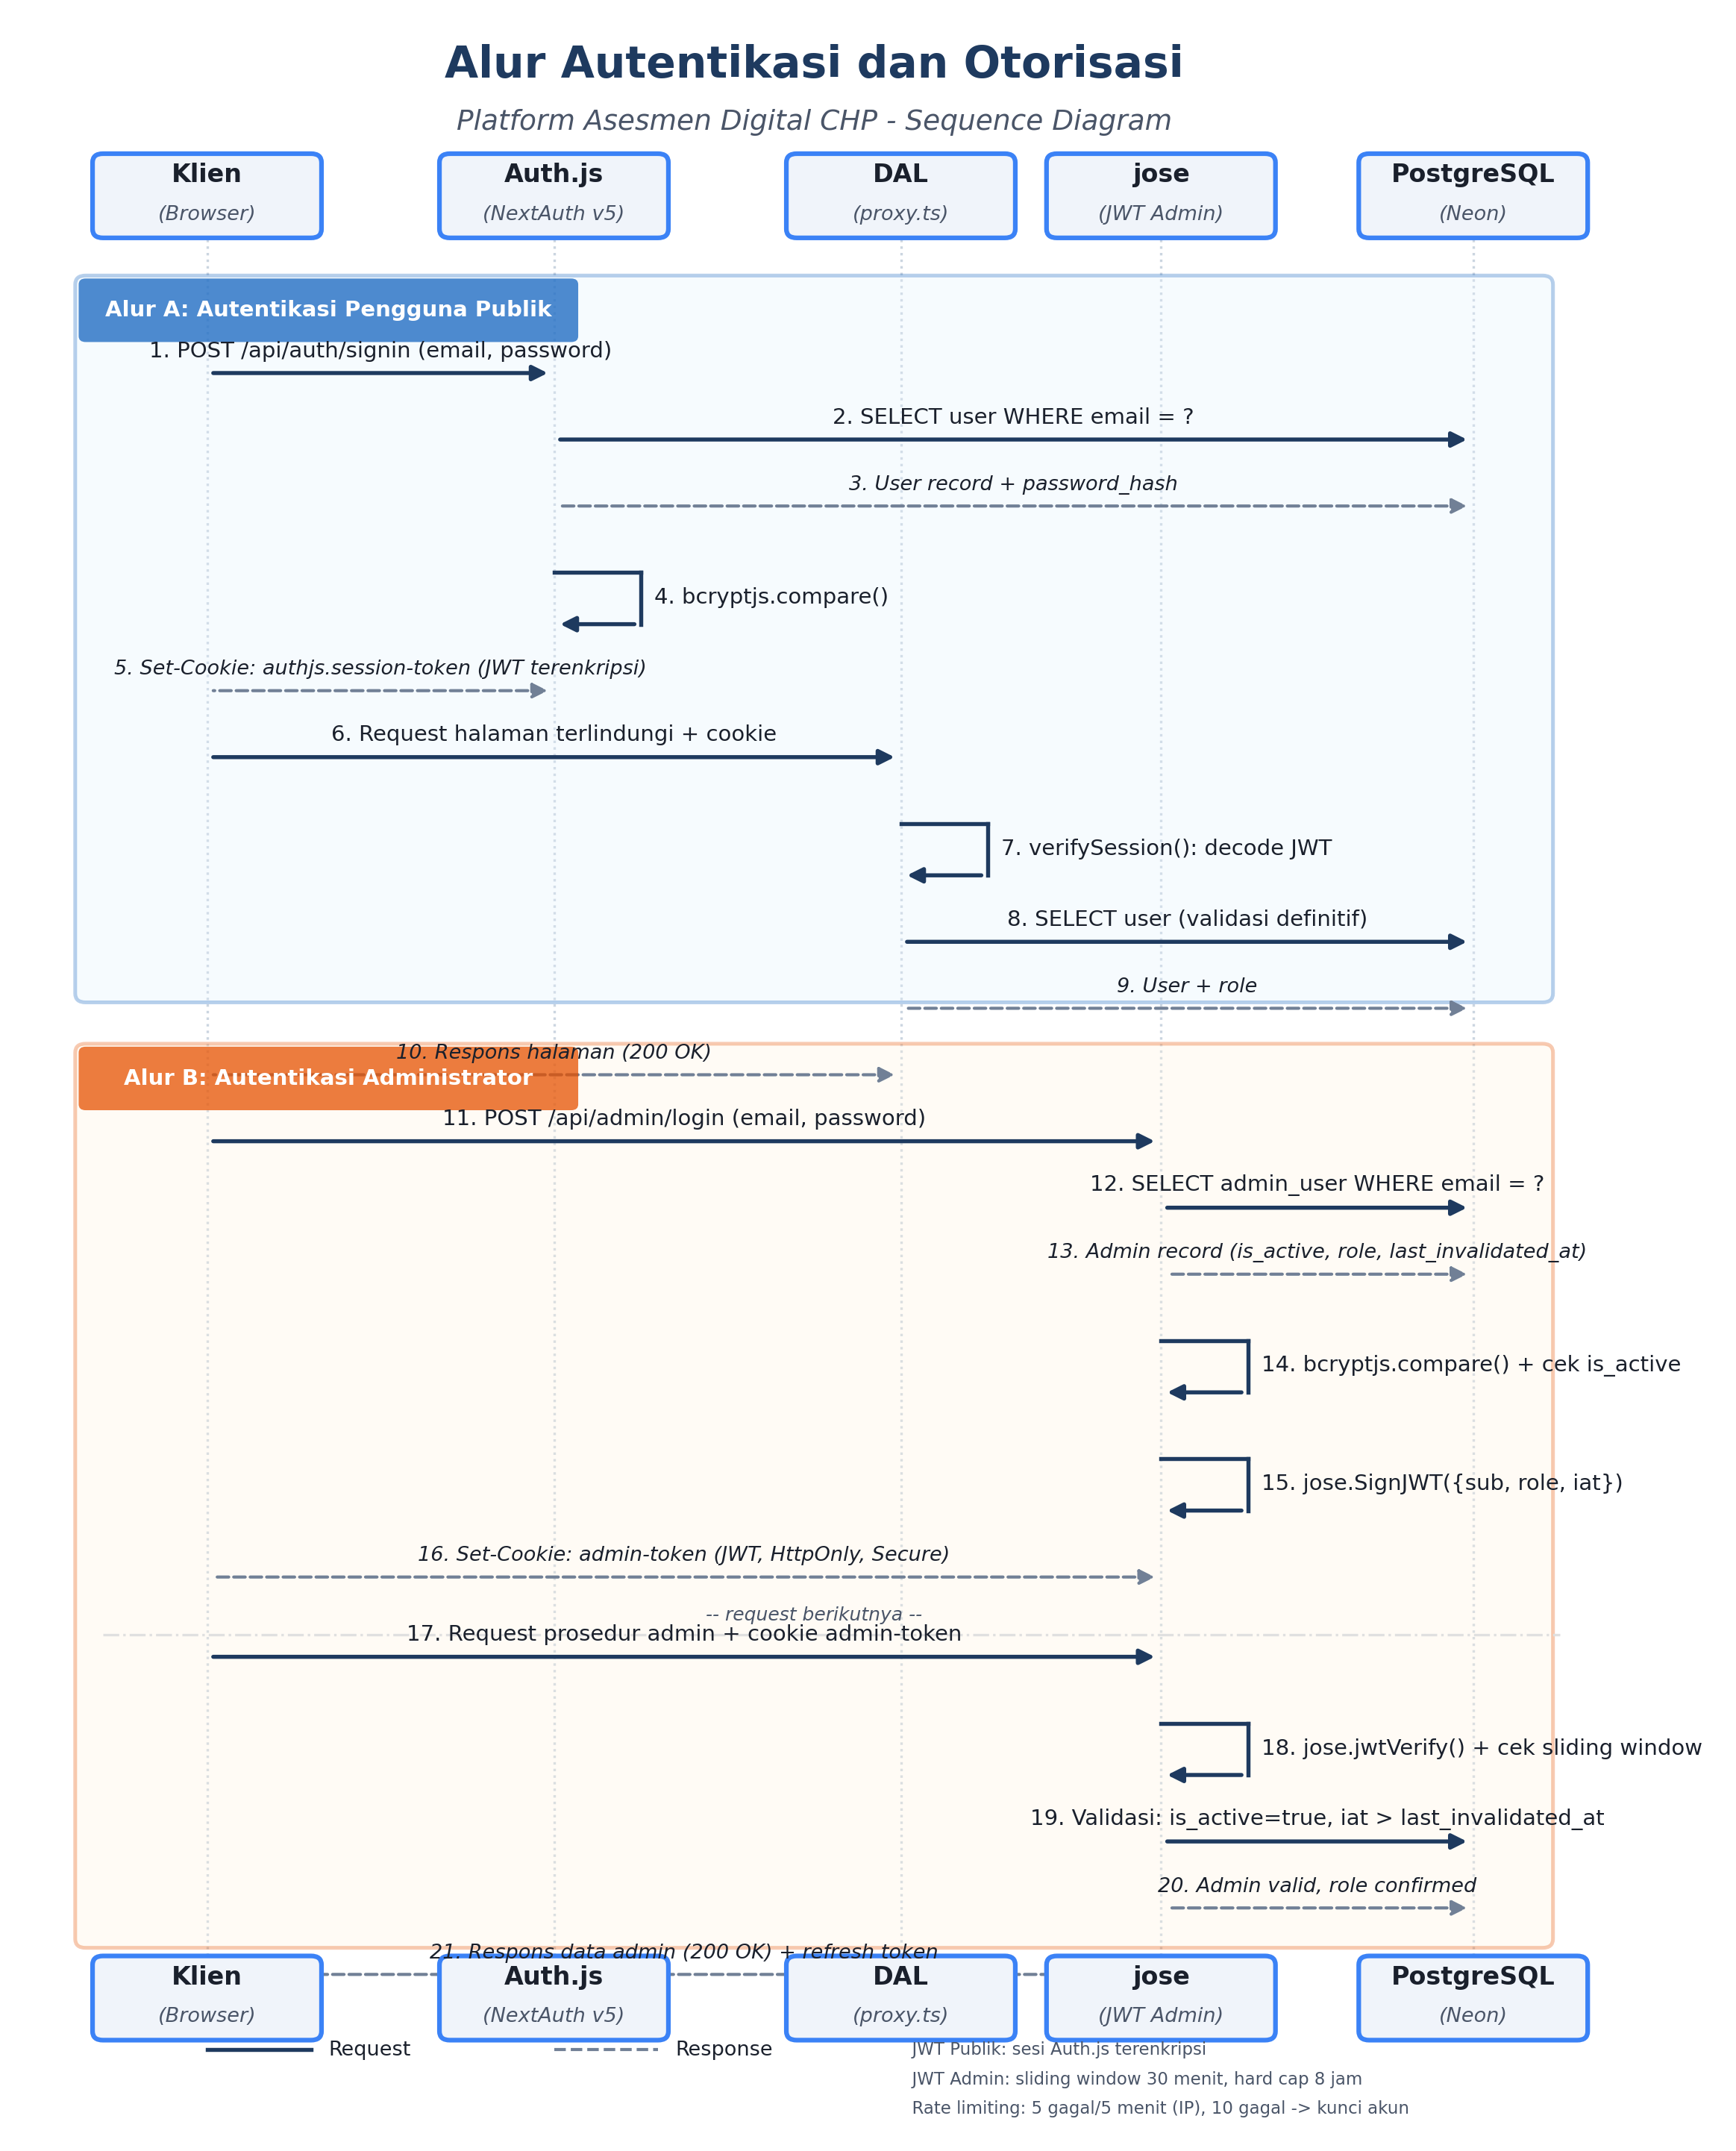
\includegraphics[width=\textwidth]{figures/gambar_2_2_alur_autentikasi.png}
  \caption{Alur Autentikasi dan Otorisasi Platform CHP (\textit{Sequence Diagram})}
  \label{fig:auth-flow}
\end{figure}

\subsection{JSON \textit{Web Token} (JWT)}
\label{subsec:jwt}

\textit{JSON Web Token} (JWT) adalah standar terbuka yang didefinisikan dalam RFC 7519 untuk mentransmisikan informasi secara aman antara pihak-pihak sebagai objek JSON yang ringkas dan mandiri (Jones, Bradley, dan Sakimura 2015). Sebuah JWT terdiri atas tiga bagian: Header (metadata \textit{token}), Payload (klaim tentang pengguna), dan Signature (tanda tangan digital).

Platform CHP mengimplementasikan sistem autentikasi ganda berbasis JWT:

\begin{enumerate}[leftmargin=2cm]
  \item \textbf{Autentikasi pengguna publik} melalui Auth.js (NextAuth v5) dengan \textit{CredentialsProvider}, di mana sesi pengguna disimpan dalam JWT terenkripsi dengan strategi sesi JWT.
  \item \textbf{Autentikasi administrator} melalui pustaka jose secara mandiri (terpisah dari Auth.js), dengan \textit{sliding window} 30 menit dan batas keras (\textit{hard cap}) 8 jam dari waktu penerbitan awal. JWT administrator disimpan dalam \textit{cookie} bernama \texttt{admin-token}.
\end{enumerate}

% [C2] Fixed: "dua peran" → empat peran with correct names
\subsection{\textit{Role-Based Access Control} (RBAC)}
\label{subsec:rbac}

\textit{Role-Based Access Control} (RBAC) adalah model kontrol akses di mana izin diberikan kepada peran tertentu, dan pengguna mendapatkan izin melalui keanggotaan dalam peran yang relevan. RBAC menerapkan prinsip hak istimewa minimal (\textit{principle of least privilege}).

Platform CHP mendefinisikan empat peran untuk pengguna panel admin melalui \textit{enum} PostgreSQL \texttt{admin\_role}:

\begin{enumerate}[leftmargin=2cm]
  \item \textbf{Super Admin} (\texttt{super\_admin}): Memiliki akses penuh terhadap semua operasi, termasuk manajemen akun admin, konfigurasi sistem, dan kemampuan menghapus data.
  \item \textbf{Admin} (\texttt{admin}): Memiliki akses untuk mengelola instrumen tes, melihat data respons sesi, dan mengekspor data penelitian, namun tidak dapat mengelola pengguna admin lain.
  \item \textbf{Psikiater} (\texttt{psychiatrist}): Memiliki akses untuk melihat hasil asesmen dan menyetujui permintaan laporan, dengan fokus pada evaluasi klinis.
  \item \textbf{Peneliti} (\texttt{researcher}): Memiliki akses baca terhadap data riset dan statistik untuk keperluan penelitian, tanpa kemampuan mengubah konfigurasi sistem.
\end{enumerate}

% [C9] Fixed: 3 → 5 middleware levels
Pemeriksaan otorisasi RBAC diimplementasikan pada lapisan \textit{middleware} prosedur tRPC menggunakan lima tingkat kontrol akses:

\begin{enumerate}[leftmargin=2cm]
  \item \texttt{publicProcedure}: tidak memerlukan autentikasi. Digunakan untuk prosedur asesmen dan hasil.
  \item \texttt{protectedProcedure}: memerlukan sesi Auth.js yang valid. Digunakan untuk operasi yang memerlukan identitas pengguna (klaim sesi, profil, riwayat).
  \item \texttt{adminProcedure}: memvalidasi JWT admin melalui jose, memeriksa status aktif dan waktu invalidasi sesi di basis data, serta menerapkan \textit{sliding window refresh}. Digunakan untuk operasi baca pada panel admin.
  \item \texttt{adminMutationProcedure}: memperluas \texttt{adminProcedure} dengan membatasi akses hanya kepada peran \texttt{super\_admin} dan \texttt{admin}. Digunakan untuk operasi tulis pada instrumen tes dan konfigurasi.
  \item \texttt{superAdminProcedure}: memperluas \texttt{adminProcedure} dengan membatasi akses secara eksklusif kepada peran \texttt{super\_admin}. Digunakan untuk manajemen akun admin dan operasi keamanan.
\end{enumerate}

% ─────────────────────────────────────────────────────────────────────────────
\section{Pengujian Perangkat Lunak}
\label{sec:pengujian}

Pengujian perangkat lunak adalah proses evaluasi dan verifikasi bahwa produk perangkat lunak melakukan apa yang seharusnya dilakukan. Pengujian yang komprehensif amat penting untuk Platform CHP mengingat kekritisan akurasi skor dalam konteks penelitian psikometri.

% --- Professor-approved: Testing methodologies (B2.1) ---
\subsection{Metodologi Pengujian}
\label{subsec:metodologi-pengujian}

Dua metodologi pengujian utama digunakan dalam proyek ini. \textit{White-box testing} (pengujian kotak putih, juga dikenal sebagai pengujian struktural) adalah teknik pengujian di mana penguji memiliki akses penuh terhadap kode sumber dan struktur internal sistem (Capote 2023; Bhat dan Khan 2021). Penguji merancang kasus uji berdasarkan pengetahuan tentang jalur eksekusi, kondisi percabangan, dan aliran data dalam kode. \textit{Black-box testing} (pengujian kotak hitam, juga dikenal sebagai pengujian fungsional atau pengujian perilaku) adalah teknik pengujian di mana penguji hanya mengetahui masukan dan keluaran yang diharapkan, tanpa akses terhadap implementasi internal (Capote 2023; Khan dan Khan 2022).

Platform CHP menggunakan pendekatan gabungan: \textit{white-box testing} diterapkan pada \textit{scoring engine} untuk memverifikasi setiap jalur komputasi (pembalikan skor, pengelompokan dimensional, penanganan kasus tepi), sedangkan \textit{black-box testing} diterapkan pada alur pengguna secara keseluruhan (mengisi asesmen, menerima hasil, mengelola instrumen). Tabel~\ref{tab:metodologi-testing} menyajikan pemetaan metodologi pengujian yang digunakan.

\begin{table}[htbp]
  \centering
  \caption{Pemetaan Metodologi Pengujian Platform CHP}
  \label{tab:metodologi-testing}
  \begin{tabularx}{\textwidth}{@{}p{2.5cm} p{2.5cm} X p{2cm}@{}}
    \toprule
    \textbf{Metodologi} & \textbf{Level} & \textbf{Komponen} & \textbf{Alat} \\
    \midrule
    \textit{White-box} & \textit{Unit} & \textit{Scoring engine}, validasi, enkripsi & Vitest \\
    \textit{White-box} & Integrasi & tRPC $\leftrightarrow$ DB, Auth $\leftrightarrow$ RBAC & Vitest \\
    \textit{Black-box} & \textit{End-to-end} & Alur asesmen, alur admin & Playwright \\
    \textit{Black-box} & Validasi & Akurasi skor vs.\ panduan manual & Vitest \\
    \bottomrule
  \end{tabularx}
\end{table}

% --- Professor-approved: Testing pyramid (B2.2) ---
\subsection{Strategi Piramida Pengujian}
\label{subsec:piramida-testing}

Strategi pengujian Platform CHP mengikuti konsep piramida pengujian (\textit{testing pyramid}) yang dipopulerkan oleh Cohn (2009). Piramida pengujian menempatkan \textit{unit test} pada dasar piramida (jumlah terbanyak, eksekusi tercepat, biaya terendah), \textit{integration test} di tengah, dan \textit{end-to-end test} di puncak (jumlah paling sedikit, eksekusi paling lambat, biaya tertinggi). Pendekatan ini memaksimalkan cakupan pengujian sembari meminimalkan waktu eksekusi dan biaya pemeliharaan (Desai, Singh, dan Amilkanthwar 2025). Gambar~\ref{fig:piramida-testing} mengilustrasikan hierarki ini.

\begin{figure}[htbp]
  \centering
  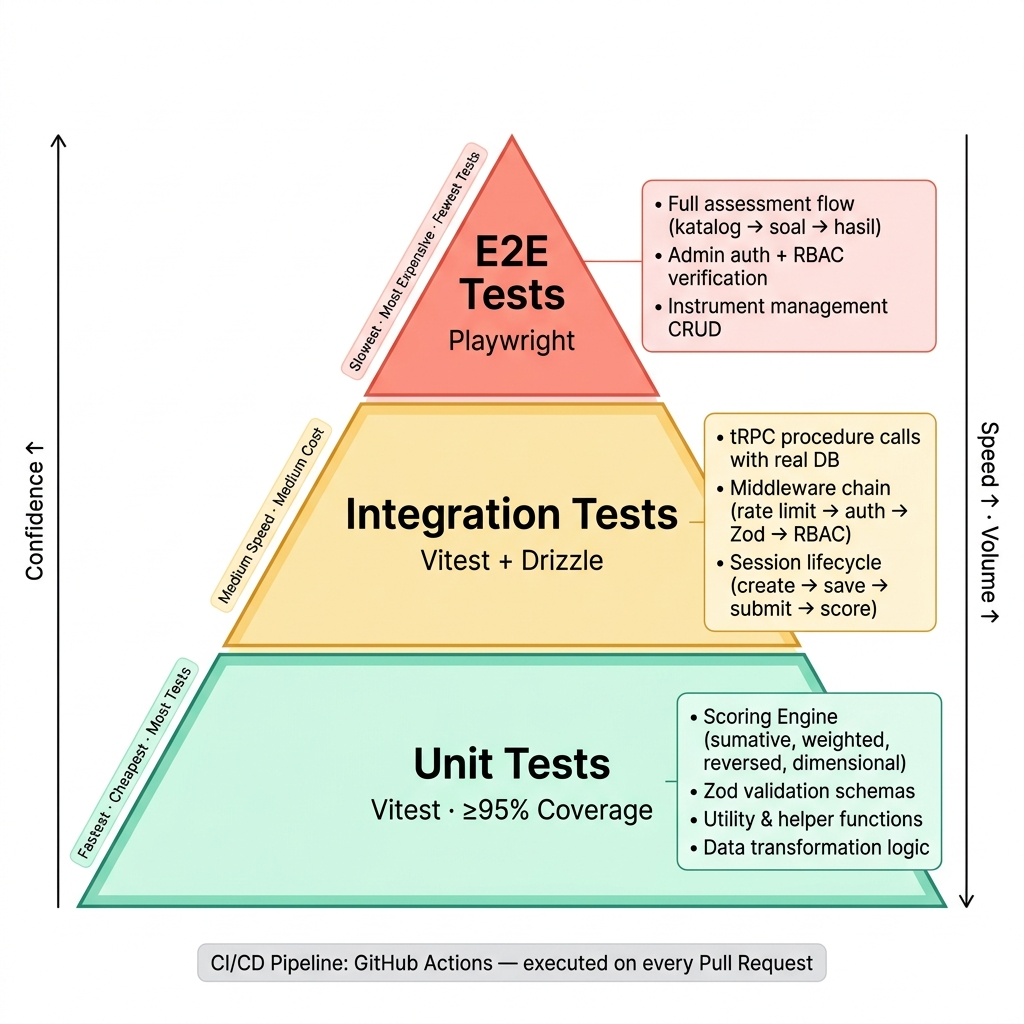
\includegraphics[width=\textwidth]{figures/gambar_2_3_piramida_pengujian.png}
  \caption{Piramida Pengujian Platform Asesmen Digital CHP}
  \label{fig:piramida-testing}
\end{figure}

% --- Professor-approved: Integration testing (B2.3) ---
\subsection{\textit{Integration Testing}}
\label{subsec:integration-testing}

\textit{Integration testing} pada Platform CHP menggunakan metodologi \textit{grey-box}: penguji mengetahui arsitektur internal (skema basis data, kontrak tRPC) namun menguji prosedur sebagai unit fungsional yang utuh. Tiga area fokus integrasi:

\begin{enumerate}[leftmargin=2cm]
  \item \textbf{tRPC $\leftrightarrow$ Basis Data}: memverifikasi bahwa prosedur tRPC menulis dan membaca data yang benar dari PostgreSQL melalui Drizzle ORM, termasuk transaksi atomik dan \textit{constraint} referensial.
  \item \textbf{Autentikasi $\leftrightarrow$ RBAC}: memverifikasi bahwa setiap tingkat \textit{middleware} (dari \texttt{publicProcedure} hingga \texttt{superAdminProcedure}) secara benar mengizinkan atau menolak akses berdasarkan peran pengguna.
  \item \textbf{Validasi Zod $\leftrightarrow$ Logika Bisnis}: memverifikasi bahwa skema masukan Zod menolak data yang tidak valid sebelum logika bisnis dieksekusi, serta bahwa pesan kesalahan yang dikembalikan informatif dan konsisten.
\end{enumerate}

% --- Professor-approved: Validation testing (B2.4) ---
\subsection{Pengujian Validasi: Akurasi Skor Otomatis}
\label{subsec:validation-testing}

Dalam konteks platform asesmen psikometri, pengujian validasi memiliki signifikansi yang melampaui pengujian perangkat lunak konvensional. Skor yang dihasilkan oleh \textit{scoring engine} harus identik dengan skor yang dihitung secara manual menggunakan panduan penilaian (\textit{scoring guide}) resmi masing-masing instrumen (Liu, Chen, dan Sun 2016). Pengujian validasi dilaksanakan dengan membandingkan keluaran \textit{scoring engine} terhadap tabel referensi yang dihitung secara manual untuk setiap instrumen, memverifikasi keidentikan skor (\textit{score identity accuracy}). Selain akurasi, efisiensi waktu juga diukur: komputasi skor otomatis yang sebelumnya memerlukan hitungan menit secara manual kini diselesaikan dalam hitungan milidetik.

\subsection{\textit{Unit Testing} dengan Vitest}
\label{subsec:vitest}

Vitest adalah \textit{framework unit testing} berbasis Vite yang dirancang khusus untuk ekosistem TypeScript/JavaScript modern. Vitest menggunakan model eksekusi yang kompatibel dengan Jest namun dengan kecepatan yang lebih tinggi berkat eksekusi langsung tanpa proses kompilasi TypeScript berulang.

% [C5] Listed all 5 exported functions
Modul \textit{scoring engine} menjadi prioritas utama \textit{unit testing} pada Platform CHP. \textit{Scoring engine} terdiri atas tiga \textit{file} dengan lima fungsi yang diekspor:

\begin{enumerate}[leftmargin=2cm]
  \item \texttt{reverseScore(rawValue, options)}: menghitung skor terbalik secara agnostik skala: $(\text{scaleMax} - \text{rawValue}) + \text{scaleMin}$.
  \item \texttt{computeScore(input)}: fungsi inti yang menangani pembalikan butir soal, penjumlahan berbobot, pengelompokan dimensional, \textit{rollup} orde kedua untuk DSR (GPIUS-2), dan komputasi \texttt{maxPossibleScore}.
  \item \texttt{lookupInterpretation(testId, totalScore, dimension?)} : mengkueri tabel \texttt{result\_interpretations} untuk pemetaan skor ke label, deskripsi, rekomendasi, dan tingkat keparahan.
  \item \texttt{validateAnswerValues(answers, questions)} : memvalidasi bahwa setiap nilai jawaban berada dalam batas opsi yang valid. Fungsi murni tanpa akses basis data.
  \item \texttt{validateCompleteness(answers, questions)} : memvalidasi bahwa semua butir soal wajib telah dijawab. Fungsi murni tanpa akses basis data.
\end{enumerate}

Tabel~\ref{tab:skenario-unit-test} menampilkan contoh skenario \textit{unit test} yang diimplementasikan.

\begin{table}[htbp]
  \centering
  \caption{Contoh Skenario \textit{Unit Test} pada \textit{Scoring Engine}}
  \label{tab:skenario-unit-test}
  \begin{tabularx}{\textwidth}{@{}p{3.5cm} X X@{}}
    \toprule
    \textbf{Fungsi} & \textbf{Kondisi Masukan} & \textbf{Hasil yang Diharapkan} \\
    \midrule
    \texttt{computeScore} (sumatif) & 5 soal dengan nilai 4, 3, 5, 2, 4 & totalScore = 18 \\
    \texttt{computeScore} (terbalik) & Soal is\_reversed=true, skala 1--5, jawaban 2 & Skor soal menjadi 4 $(5+1-2)$ \\
    \texttt{computeScore} (dimensional) & 10 soal: 5 dimensi A, 5 dimensi B & dimensionScores terpisah per dimensi \\
    \texttt{\seqsplit{validateCompleteness}} & Satu soal wajib belum dijawab & valid = false, missingQuestionIds berisi ID soal \\
    \bottomrule
  \end{tabularx}
\end{table}

\subsection{\textit{End-to-End Testing} dengan Playwright}
\label{subsec:playwright}

Playwright adalah \textit{framework} otomasi \textit{browser} yang dikembangkan oleh Microsoft untuk E2E \textit{testing}. Tiga alur kritis yang menjadi prioritas E2E \textit{testing} adalah: (1) alur asesmen penuh dari katalog hingga halaman hasil; (2) alur autentikasi admin termasuk \textit{redirect} otomatis; dan (3) alur manajemen instrumen dari pembuatan hingga publikasi.

% [C6] Fixed: "4 gate sequential" → 2 parallel jobs
\subsection{CI/CD dengan GitHub Actions}
\label{subsec:cicd}

\textit{Continuous Integration/Continuous Deployment} (CI/CD) menghilangkan proses integrasi dan \textit{deployment} manual yang rawan kesalahan. Platform CHP mengimplementasikan \textit{pipeline} CI/CD menggunakan GitHub Actions yang diaktifkan pada setiap \textit{pull request} dan \textit{push} ke cabang utama \texttt{master}.

\textit{Pipeline} terdiri atas dua \textit{job} yang berjalan secara paralel:

\begin{enumerate}[leftmargin=2cm]
  \item \textbf{\textit{Job} 1: \texttt{build-and-test}}: menjalankan tiga \textit{gate} secara berurutan:
  \begin{enumerate}
    \item Pemeriksaan \textit{linting} (ESLint): memastikan konsistensi gaya kode.
    \item Pemeriksaan \textit{type checking} (TypeScript \textit{Compiler} dengan \textit{strict mode}): memastikan tidak ada kesalahan tipe.
    \item Proses \textit{build} produksi (Next.js): memastikan aplikasi dapat dikompilasi untuk lingkungan produksi.
  \end{enumerate}
  \item \textbf{\textit{Job} 2: \texttt{test}}: menjalankan \textit{unit test} (Vitest) secara paralel dengan \textit{Job} 1, sehingga hasil pengujian tersedia lebih cepat tanpa menunggu proses \textit{build} selesai.
\end{enumerate}

Sebuah \textit{pull request} tidak dapat di-\textit{merge} ke cabang utama apabila salah satu dari kedua \textit{job} tersebut gagal. Gambar~\ref{fig:cicd-pipeline} mengilustrasikan diagram alur \textit{pipeline}.

\begin{figure}[htbp]
  \centering
  \includegraphics[width=\textwidth]{figures/gambar_2_4_pipeline_cicd.png}
  \caption{Diagram Alur \textit{Pipeline} CI/CD Platform CHP (\textit{Activity Diagram})}
  \label{fig:cicd-pipeline}
\end{figure}

% ─────────────────────────────────────────────────────────────────────────────
\section{Keamanan dan Privasi Data}
\label{sec:keamanan}

Platform yang menangani data psikologis sensitif memiliki kewajiban keamanan yang lebih tinggi dibandingkan aplikasi umum.

\subsection{OWASP \textit{Top Ten}}
\label{subsec:owasp}

OWASP \textit{Top Ten} menjadi standar acuan \textit{de-facto} dalam komunitas keamanan perangkat lunak (OWASP Foundation 2026). Platform CHP mengimplementasikan mitigasi terhadap risiko yang paling relevan:

\begin{enumerate}[leftmargin=2cm]
  \item A01 \textit{Broken Access Control}: Dimitigasi melalui RBAC lima tingkat dan pemeriksaan otorisasi pada setiap prosedur tRPC yang dilindungi.
  % [C4] Fixed: bcrypt → bcryptjs
  \item A02 \textit{Cryptographic Failures}: Data \textit{in transit} dienkripsi via TLS/HTTPS. Data \textit{at rest} dienkripsi oleh infrastruktur Neon PostgreSQL.
  \item A03 \textit{Injection}: Dicegah melalui Drizzle ORM yang menggunakan \textit{parameterized queries}. Seluruh masukan pengguna divalidasi menggunakan skema Zod.
  \item A07 \textit{Identification and Authentication Failures}: Dimitigasi melalui JWT yang aman, \textit{password hashing} menggunakan bcryptjs (\textit{pure JavaScript}, tanpa \textit{native binding}) dengan \textit{cost factor} 12, dan proteksi \textit{brute force} melalui \textit{rate limiting}.
\end{enumerate}

\subsection{\textit{Rate Limiting} dan Perlindungan API}
\label{subsec:rate-limiting}

Platform CHP mengimplementasikan \textit{rate limiting} berlapis:

\begin{enumerate}[leftmargin=2cm]
  \item \textbf{Upstash Redis} (\texttt{@upstash/ratelimit}): diterapkan pada lapisan \textit{proxy} untuk membatasi permintaan API secara global. Kompatibel dengan lingkungan \textit{serverless} Vercel.
  \item \textbf{\textit{In-memory rate limiter}} untuk \textit{login} admin: dua tingkat pembatasan, yaitu berbasis IP (5 kegagalan dalam 5 menit) dan berbasis akun (10 kegagalan yang mengunci akun hingga dibuka oleh \texttt{super\_admin}).
\end{enumerate}

\subsection{Undang-Undang Perlindungan Data Pribadi}
\label{subsec:uu-pdp}

Undang-Undang Nomor 27 Tahun 2022 tentang Perlindungan Data Pribadi (UU PDP) mengamanatkan penerapan prinsip \textit{privacy by design} dan minimisasi data (Rebong, Hambali, dan Timothy 2025). Platform CHP mengimplementasikan prinsip-prinsip UU PDP melalui empat mekanisme:

\begin{enumerate}[leftmargin=2cm]
  \item Sesi asesmen anonim tanpa memerlukan akun pengguna.
  \item Penyamaran alamat IP: alamat IP di-\textit{hash} satu arah sebelum disimpan.
  \item Persetujuan eksplisit melalui modul \texttt{consents} yang terpisah.
  \item Enkripsi surel peserta menggunakan AES-256-GCM dalam tabel \texttt{guest\_leads} yang terisolasi.
\end{enumerate}
